% Options for packages loaded elsewhere
\PassOptionsToPackage{unicode}{hyperref}
\PassOptionsToPackage{hyphens}{url}
%
\documentclass[
  ignorenonframetext,
]{beamer}
\title{Spatial modeling with \texttt{INLA} and \texttt{inlabru}}
\subtitle{University of Zurich, March, 2022}
\author{Instructor: Sara Martino}
\date{}
\institute{Department of Mathematical Science (NTNU)}

\usepackage{pgfpages}
\setbeamertemplate{caption}[numbered]
\setbeamertemplate{caption label separator}{: }
\setbeamercolor{caption name}{fg=normal text.fg}
\beamertemplatenavigationsymbolsempty
% Prevent slide breaks in the middle of a paragraph
\widowpenalties 1 10000
\raggedbottom
\setbeamertemplate{part page}{
  \centering
  \begin{beamercolorbox}[sep=16pt,center]{part title}
    \usebeamerfont{part title}\insertpart\par
  \end{beamercolorbox}
}
\setbeamertemplate{section page}{
  \centering
  \begin{beamercolorbox}[sep=12pt,center]{part title}
    \usebeamerfont{section title}\insertsection\par
  \end{beamercolorbox}
}
\setbeamertemplate{subsection page}{
  \centering
  \begin{beamercolorbox}[sep=8pt,center]{part title}
    \usebeamerfont{subsection title}\insertsubsection\par
  \end{beamercolorbox}
}
\AtBeginPart{
  \frame{\partpage}
}
\AtBeginSection{
  \ifbibliography
  \else
    \frame{\sectionpage}
  \fi
}
\AtBeginSubsection{
  \frame{\subsectionpage}
}
\usepackage{amsmath,amssymb}
\usepackage{lmodern}
\usepackage{iftex}
\ifPDFTeX
  \usepackage[T1]{fontenc}
  \usepackage[utf8]{inputenc}
  \usepackage{textcomp} % provide euro and other symbols
\else % if luatex or xetex
  \usepackage{unicode-math}
  \defaultfontfeatures{Scale=MatchLowercase}
  \defaultfontfeatures[\rmfamily]{Ligatures=TeX,Scale=1}
\fi
\usetheme[]{Singapore}
\usefonttheme{serif}
% Use upquote if available, for straight quotes in verbatim environments
\IfFileExists{upquote.sty}{\usepackage{upquote}}{}
\IfFileExists{microtype.sty}{% use microtype if available
  \usepackage[]{microtype}
  \UseMicrotypeSet[protrusion]{basicmath} % disable protrusion for tt fonts
}{}
\makeatletter
\@ifundefined{KOMAClassName}{% if non-KOMA class
  \IfFileExists{parskip.sty}{%
    \usepackage{parskip}
  }{% else
    \setlength{\parindent}{0pt}
    \setlength{\parskip}{6pt plus 2pt minus 1pt}}
}{% if KOMA class
  \KOMAoptions{parskip=half}}
\makeatother
\usepackage{xcolor}
\IfFileExists{xurl.sty}{\usepackage{xurl}}{} % add URL line breaks if available
\IfFileExists{bookmark.sty}{\usepackage{bookmark}}{\usepackage{hyperref}}
\hypersetup{
  pdftitle={Spatial modeling with INLA and inlabru},
  pdfauthor={Instructor: Sara Martino},
  hidelinks,
  pdfcreator={LaTeX via pandoc}}
\urlstyle{same} % disable monospaced font for URLs
\newif\ifbibliography
\usepackage{color}
\usepackage{fancyvrb}
\newcommand{\VerbBar}{|}
\newcommand{\VERB}{\Verb[commandchars=\\\{\}]}
\DefineVerbatimEnvironment{Highlighting}{Verbatim}{commandchars=\\\{\}}
% Add ',fontsize=\small' for more characters per line
\usepackage{framed}
\definecolor{shadecolor}{RGB}{248,248,248}
\newenvironment{Shaded}{\begin{snugshade}}{\end{snugshade}}
\newcommand{\AlertTok}[1]{\textcolor[rgb]{0.94,0.16,0.16}{#1}}
\newcommand{\AnnotationTok}[1]{\textcolor[rgb]{0.56,0.35,0.01}{\textbf{\textit{#1}}}}
\newcommand{\AttributeTok}[1]{\textcolor[rgb]{0.77,0.63,0.00}{#1}}
\newcommand{\BaseNTok}[1]{\textcolor[rgb]{0.00,0.00,0.81}{#1}}
\newcommand{\BuiltInTok}[1]{#1}
\newcommand{\CharTok}[1]{\textcolor[rgb]{0.31,0.60,0.02}{#1}}
\newcommand{\CommentTok}[1]{\textcolor[rgb]{0.56,0.35,0.01}{\textit{#1}}}
\newcommand{\CommentVarTok}[1]{\textcolor[rgb]{0.56,0.35,0.01}{\textbf{\textit{#1}}}}
\newcommand{\ConstantTok}[1]{\textcolor[rgb]{0.00,0.00,0.00}{#1}}
\newcommand{\ControlFlowTok}[1]{\textcolor[rgb]{0.13,0.29,0.53}{\textbf{#1}}}
\newcommand{\DataTypeTok}[1]{\textcolor[rgb]{0.13,0.29,0.53}{#1}}
\newcommand{\DecValTok}[1]{\textcolor[rgb]{0.00,0.00,0.81}{#1}}
\newcommand{\DocumentationTok}[1]{\textcolor[rgb]{0.56,0.35,0.01}{\textbf{\textit{#1}}}}
\newcommand{\ErrorTok}[1]{\textcolor[rgb]{0.64,0.00,0.00}{\textbf{#1}}}
\newcommand{\ExtensionTok}[1]{#1}
\newcommand{\FloatTok}[1]{\textcolor[rgb]{0.00,0.00,0.81}{#1}}
\newcommand{\FunctionTok}[1]{\textcolor[rgb]{0.00,0.00,0.00}{#1}}
\newcommand{\ImportTok}[1]{#1}
\newcommand{\InformationTok}[1]{\textcolor[rgb]{0.56,0.35,0.01}{\textbf{\textit{#1}}}}
\newcommand{\KeywordTok}[1]{\textcolor[rgb]{0.13,0.29,0.53}{\textbf{#1}}}
\newcommand{\NormalTok}[1]{#1}
\newcommand{\OperatorTok}[1]{\textcolor[rgb]{0.81,0.36,0.00}{\textbf{#1}}}
\newcommand{\OtherTok}[1]{\textcolor[rgb]{0.56,0.35,0.01}{#1}}
\newcommand{\PreprocessorTok}[1]{\textcolor[rgb]{0.56,0.35,0.01}{\textit{#1}}}
\newcommand{\RegionMarkerTok}[1]{#1}
\newcommand{\SpecialCharTok}[1]{\textcolor[rgb]{0.00,0.00,0.00}{#1}}
\newcommand{\SpecialStringTok}[1]{\textcolor[rgb]{0.31,0.60,0.02}{#1}}
\newcommand{\StringTok}[1]{\textcolor[rgb]{0.31,0.60,0.02}{#1}}
\newcommand{\VariableTok}[1]{\textcolor[rgb]{0.00,0.00,0.00}{#1}}
\newcommand{\VerbatimStringTok}[1]{\textcolor[rgb]{0.31,0.60,0.02}{#1}}
\newcommand{\WarningTok}[1]{\textcolor[rgb]{0.56,0.35,0.01}{\textbf{\textit{#1}}}}
\setlength{\emergencystretch}{3em} % prevent overfull lines
\providecommand{\tightlist}{%
  \setlength{\itemsep}{0pt}\setlength{\parskip}{0pt}}
\setcounter{secnumdepth}{-\maxdimen} % remove section numbering
% handouts
\usepackage{handoutWithNotes} 
% put 3 slides on 1 page with space for notes
%\pgfpagesuselayout{3 on 1 with notes}[a4paper, border shrink=5mm]


% smaller space in between lines in toc
\makeatletter
\patchcmd{\beamer@sectionintoc}{\vskip1.5em}{\vskip0.5em}{}{}
\makeatother


% two columns environmnt
\newenvironment{cols}[1][]{}{}

\newenvironment{col}[1]{\begin{minipage}{#1}\ignorespaces}{%
\end{minipage}
\ifhmode\unskip\fi
\aftergroup\useignorespacesandallpars}

\def\useignorespacesandallpars#1\ignorespaces\fi{%
#1\fi\ignorespacesandallpars}

\makeatletter
\def\ignorespacesandallpars{%
  \@ifnextchar\par
    {\expandafter\ignorespacesandallpars\@gobble}%
    {}%
}
\makeatother

%% logo on first page
\titlegraphic{\centering 
\includegraphics[width=6cm]{log_ntnu.jpg}}
\ifLuaTeX
  \usepackage{selnolig}  % disable illegal ligatures
\fi

\begin{document}
\frame{\titlepage}

\begin{frame}[allowframebreaks]
  \tableofcontents[hideallsubsections]
\end{frame}
\begin{frame}
\end{frame}

\hypertarget{model-choice-and-model-assessmentvalidation}{%
\section{Model choice and model
assessment/validation}\label{model-choice-and-model-assessmentvalidation}}

\begin{frame}{Introduction}
\protect\hypertarget{introduction}{}
We have now seen some fancy modelling approaches

\pause

How can we assess the models and choose between them?

\begin{itemize}
\tightlist
\item
  Rather underdeveloped in statistical literature; Many suggestions; no
  clear ``yes, this is how it should be done''
\end{itemize}
\end{frame}

\begin{frame}{Model choice and assessment}
\protect\hypertarget{model-choice-and-assessment}{}
\begin{itemize}
\item
  \textbf{Model assessment} is the art and science of evaluating how
  well a model and/or estimate agrees with observed reality, and of how
  useful it for specific purposes

  \begin{itemize}
  \tightlist
  \item
    Simple models -summary characteristics
  \item
    Complex models - assessing variability in space
  \item
    All models - prediction ability; calibrated uncertainty
  \end{itemize}
\item
  \textbf{Model choice} - which covariate and random effects to include
\item
  \textbf{Model comparison} - which model is ``better?''
\end{itemize}
\end{frame}

\begin{frame}{Model choice}
\protect\hypertarget{model-choice}{}
INLA can compute the following quantities:

\begin{itemize}
\item
  Marginal likelihood \(\Rightarrow\) Bayes factors
\item
  Deviance information criterion (DIC)
\item
  Widely applicable information criterion (WAIC)
\end{itemize}
\end{frame}

\begin{frame}{General advice}
\protect\hypertarget{general-advice}{}
\begin{itemize}
\item
  We have little experience with practical usage of them for complex
  spatial models
\item
  It is not clear what they actually mean in the context of the models
  we look at here
\item
  Advice: use them cautiously
\item
  Less adventurous if you are comparing models with only different
  numbers of covariates - and ``the rest'' is the same:

  \begin{itemize}
  \tightlist
  \item
    Use the same mesh in the models you compare (do not treat the mesh
    resolution as a model choice!)
  \end{itemize}
\end{itemize}
\end{frame}

\begin{frame}[fragile]{Marginal likelihood}
\protect\hypertarget{marginal-likelihood}{}
\small

\begin{Shaded}
\begin{Highlighting}[]
\NormalTok{result }\OtherTok{=} \FunctionTok{inla}\NormalTok{(...,}
              \AttributeTok{control.compute=}\FunctionTok{list}\NormalTok{(}\AttributeTok{mlik=}\ConstantTok{TRUE}\NormalTok{))}

\NormalTok{result }\OtherTok{=} \FunctionTok{bru}\NormalTok{(...,}\AttributeTok{options =} \FunctionTok{list}\NormalTok{(}\AttributeTok{control.compute =} 
                                  \FunctionTok{list}\NormalTok{(}\AttributeTok{mlik =} \ConstantTok{TRUE}\NormalTok{)))}
\end{Highlighting}
\end{Shaded}

\normalsize

\begin{itemize}
\item
  Calculates \(\log(\pi(\boldsymbol{y}))\)
\item
  Can calculate Bayes factors through differences in value
\item
  \textbf{NB:} Problematic for intrinsic models
\end{itemize}
\end{frame}

\begin{frame}[fragile]{Deviance information criterion}
\protect\hypertarget{deviance-information-criterion}{}
\small

\begin{Shaded}
\begin{Highlighting}[]
\NormalTok{result }\OtherTok{=} \FunctionTok{inla}\NormalTok{(...,}
              \AttributeTok{control.compute=}\FunctionTok{list}\NormalTok{(}\AttributeTok{dic=}\ConstantTok{TRUE}\NormalTok{))}

\NormalTok{result }\OtherTok{=} \FunctionTok{bru}\NormalTok{(...,}\AttributeTok{options =} \FunctionTok{list}\NormalTok{(}\AttributeTok{control.compute =} 
                                  \FunctionTok{list}\NormalTok{(}\AttributeTok{dic =} \ConstantTok{TRUE}\NormalTok{)))}
\end{Highlighting}
\end{Shaded}

\normalsize

\hfill\break
DIC is a measure of complexity and fit. It is used to compare complex
hierarchical models and is defined as:

\[
\text{DIC} = \overline{D} + p_D
\]

where \(\overline{D}\) is the posterior mean of the deviance and \(p_D\)
is the effective number of parameters. Smaller values of the DIC
indicate a better trade-off between complexity and fit of the model.
\end{frame}

\begin{frame}[fragile]{Widely applicable information criterion (WAIC)}
\protect\hypertarget{widely-applicable-information-criterion-waic}{}
\small

\begin{Shaded}
\begin{Highlighting}[]
\NormalTok{result }\OtherTok{=} \FunctionTok{inla}\NormalTok{(...,}
              \AttributeTok{control.compute=}\FunctionTok{list}\NormalTok{(}\AttributeTok{waic=}\ConstantTok{TRUE}\NormalTok{))}

\NormalTok{result }\OtherTok{=} \FunctionTok{bru}\NormalTok{(...,}\AttributeTok{options =} \FunctionTok{list}\NormalTok{(}\AttributeTok{control.compute =} 
                                  \FunctionTok{list}\NormalTok{(}\AttributeTok{waic =} \ConstantTok{TRUE}\NormalTok{)))}
\end{Highlighting}
\end{Shaded}

\normalsize

\begin{itemize}
\item
  WAIC is like DIC just newer, and perhaps better
\item
  See \emph{``Understanding predictive information criteria for Bayesian
  models''} (2013) by Andrew Gelman, Jessica Hwang, and Aki Vehtari
\end{itemize}
\end{frame}

\begin{frame}[fragile]{Model assessment with cross-validated scores}
\protect\hypertarget{model-assessment-with-cross-validated-scores}{}
Posterior predictive distributions can be used for model assessment and
model selection.

Full cross-validation or out-of-sample validation is expensive.

\texttt{R-INLA} provides two leave-one-out crossvalidation quantities:

\begin{itemize}
\item
  \textbf{Conditional predictive ordinate}
\item
  \textbf{Probability integral transform}
\end{itemize}
\end{frame}

\begin{frame}[fragile]{Conditional predictive ordinate}
\protect\hypertarget{conditional-predictive-ordinate}{}
\small

\begin{Shaded}
\begin{Highlighting}[]
\NormalTok{result }\OtherTok{=} \FunctionTok{inla}\NormalTok{(...,}
              \AttributeTok{control.compute=}\FunctionTok{list}\NormalTok{(}\AttributeTok{cpo=}\ConstantTok{TRUE}\NormalTok{))}

\NormalTok{result }\OtherTok{=} \FunctionTok{bru}\NormalTok{(...,}\AttributeTok{options =} \FunctionTok{list}\NormalTok{(}\AttributeTok{control.compute =} 
                                  \FunctionTok{list}\NormalTok{(}\AttributeTok{cpo =} \ConstantTok{TRUE}\NormalTok{)))}
\end{Highlighting}
\end{Shaded}

\normalsize

\begin{itemize}
\item
  Measures fit through the predictive density
  \(\pi(y_i^{obs}\mid\boldsymbol{y}_{-i})\)
\item
  Basically, Bayesian hold-one out
\item
  Easy to compute in the INLA-approach
\item
  Possible failure (\$cpo\$failure)
\item
  See \emph{Posterior and Cross-validatory Predictive Checks: A
  Comparison of MCMC and INLA} (2009) by Held, Schr\{"o\}dle and Rue
\end{itemize}
\end{frame}

\begin{frame}{Proper scoring rule based on CPO}
\protect\hypertarget{proper-scoring-rule-based-on-cpo}{}
A predictive score is proper if its expected value is minimised under
the true distribution.

\begin{itemize}
\tightlist
\item
  The \textbf{log-CPO-score} \[
  \text{logCPO} = -\sum_{i = 1}^n\log(\text{CPO}_i)  = -\sum_{i = 1}^n\log[p(y_i^{\text{obs}}|y_j^\text{obs}, j\neq i)]
  \]
\end{itemize}

is a strictly proper scoring rule.

\begin{itemize}
\item
  The logCPO score encourages appropriate prediction uncertainty; bias,
  overconfidence, and underconfidence all increase the score.
\item
  \(2\text{logCPO}\) is similar in scale to DIC and WAIC but has a clear
  cross validation prediction interpretation.
\end{itemize}
\end{frame}

\begin{frame}{Pairwise observasion CPO scores}
\protect\hypertarget{pairwise-observasion-cpo-scores}{}
\begin{itemize}
\item
  The aggregated logCPO score hides information
\item
  Model comparison for predictions is a pairwise comparison problem for
  each individual observation!
\item
  Compute the collection of pairwise logCPO differences for two models
\item
  Inspect the empirical score difference distribution; is it consitently
  positive/negative?
\item
  Inspect the spatial pattern of the score differences
\end{itemize}
\end{frame}

\begin{frame}[fragile]{Probability integral transform}
\protect\hypertarget{probability-integral-transform}{}
\small

\begin{Shaded}
\begin{Highlighting}[]
\NormalTok{result }\OtherTok{=} \FunctionTok{inla}\NormalTok{(...,}
              \AttributeTok{control.compute=}\FunctionTok{list}\NormalTok{(}\AttributeTok{pit=}\ConstantTok{TRUE}\NormalTok{))}

\NormalTok{result }\OtherTok{=} \FunctionTok{bru}\NormalTok{(...,}\AttributeTok{options =} \FunctionTok{list}\NormalTok{(}\AttributeTok{control.compute =} 
                                  \FunctionTok{list}\NormalTok{(}\AttributeTok{pit =} \ConstantTok{TRUE}\NormalTok{)))}
\end{Highlighting}
\end{Shaded}

\normalsize

\begin{itemize}
\tightlist
\item
  Given by
\end{itemize}

\[
\text{Prob}(Y_i \leq y_i^{obs} \mid \boldsymbol{y}_{-i})
\]
\end{frame}

\begin{frame}{PIT: assessing prediction bias, scale and shape}
\protect\hypertarget{pit-assessing-prediction-bias-scale-and-shape}{}
\begin{itemize}
\item
  A direct consequence of the PIT definition is that under the true
  model, each \(PIT_i\) value is a sample of a uniform distribution on
  {[}0, 1{]}.
\item
  The usual plotting method for PIT is a histogram.
\item
  For models with too small predictive variance, the histogram tends to
  increase toward 0 and 1.
\item
  For models with too large predictive variance, the histogram tends to
  have peak in the middle.
\item
  For incorrectly skewed predictions, the PIT histogram will tend to be
  skewed.
\item
  Unfortunately, that doesn't necessarily imply that overfitting and
  oversmoothing can be detected and/or correctly diagnosed.
\end{itemize}
\end{frame}

\hypertarget{advanced-features}{%
\section{Advanced features}\label{advanced-features}}

\begin{frame}[fragile]{Useful features}
\protect\hypertarget{useful-features}{}
There are several features that can be used to extend the standard
models in \texttt{R-INLA} (and \texttt{inlabru})

\begin{itemize}
\item
  Replicate
\item
  Group
\item
  Copy
\item
  Multiple likelihoods
\item
  Generic precision matrices (\texttt{rgeneric})
\end{itemize}

\textbf{Main goals}

\begin{itemize}
\tightlist
\item
  know about the features
\item
  be exposed to the ideas
\end{itemize}
\end{frame}

\hypertarget{featurereplicate}{%
\section{Feature:Replicate}\label{featurereplicate}}

\begin{frame}[fragile]{Feature: \texttt{replicate}}
\protect\hypertarget{feature-replicate}{}
\texttt{replicate} generates iid replicates from the same f\(()\)-model
with the same hyperparameters.\\
\strut \\
If \(\bf{x}\mid\bf{\theta} \sim \text{AR}(1)\), then \text{nrep=3},
makes \[
\bf{x} = ({\bf x}_{1}, {\bf x}_{2}, {\bf x}_{3})
\] with mutually independent \(\bf{x}_{i}\)'s from AR\((1)\) with the
same \(\bf{\theta}\)

\begin{Shaded}
\begin{Highlighting}[]
    \FunctionTok{f}\NormalTok{(..., }\AttributeTok{replicate =}\NormalTok{ r [, }\AttributeTok{nrep =}\NormalTok{ nr ])}
\end{Highlighting}
\end{Shaded}

where replicate are integers \(1, 2, \ldots,\) etc
\end{frame}

\begin{frame}{Example}
\protect\hypertarget{example}{}
\[
\begin{aligned}
y^1_i & \sim\text{Poisson}(\lambda^1_i), & i = 1,\dots,n_1\\
y^2_i & \sim\text{Poisson}(\lambda^2_i), & i = 1,\dots,n_2\\
\\
\log(\lambda^1_i) & = \mu_1 + u^1_i\\
\log(\lambda^2_i)  & = \mu_2 + u^2_i\\
\end{aligned}
\] and \({\bf u}^1\) and \({\bf u}^2\) are two replicates of the same
AR1 model (they share the same parameters)
\end{frame}

\begin{frame}[fragile]{Example : simulate data}
\protect\hypertarget{example-simulate-data}{}
\footnotesize

\begin{Shaded}
\begin{Highlighting}[]
\CommentTok{\# Simulate data {-} 2 groups with same AR1 param}
\NormalTok{n }\OtherTok{=} \DecValTok{100}
\NormalTok{rho }\OtherTok{\textless{}{-}} \FloatTok{0.8}
\NormalTok{mu }\OtherTok{=} \FunctionTok{c}\NormalTok{(}\DecValTok{1}\NormalTok{,}\SpecialCharTok{{-}}\DecValTok{1}\NormalTok{)}
\NormalTok{x1 }\OtherTok{=} \FunctionTok{arima.sim}\NormalTok{(}\AttributeTok{n=}\NormalTok{n, }\AttributeTok{model=}\FunctionTok{list}\NormalTok{(}\AttributeTok{ar=}\FunctionTok{c}\NormalTok{(rho))) }\SpecialCharTok{+}\NormalTok{ mu[}\DecValTok{1}\NormalTok{]}
\NormalTok{x2 }\OtherTok{=} \FunctionTok{arima.sim}\NormalTok{(}\AttributeTok{n=}\NormalTok{n, }\AttributeTok{model=}\FunctionTok{list}\NormalTok{(}\AttributeTok{ar=}\FunctionTok{c}\NormalTok{(rho))) }\SpecialCharTok{+}\NormalTok{ mu[}\DecValTok{2}\NormalTok{]}
\CommentTok{\# generate Poisson observations}
\NormalTok{y1 }\OtherTok{=} \FunctionTok{rpois}\NormalTok{(n, }\AttributeTok{lambda =} \FunctionTok{exp}\NormalTok{(x1))}
\NormalTok{y2 }\OtherTok{=} \FunctionTok{rpois}\NormalTok{(n, }\AttributeTok{lambda =} \FunctionTok{exp}\NormalTok{(x2))}

\NormalTok{df\_groups }\OtherTok{\textless{}{-}} \FunctionTok{data.frame}\NormalTok{(}\AttributeTok{y =} \FunctionTok{c}\NormalTok{(y1, y2),}
                        \AttributeTok{t =} \FunctionTok{rep}\NormalTok{(}\DecValTok{1}\SpecialCharTok{:}\NormalTok{n, }\DecValTok{2}\NormalTok{),}
                        \AttributeTok{repl =} \FunctionTok{rep}\NormalTok{(}\DecValTok{1}\SpecialCharTok{:}\DecValTok{2}\NormalTok{, }\AttributeTok{each =}\NormalTok{ n),}
                        \AttributeTok{int =} \FunctionTok{rep}\NormalTok{(}\DecValTok{0}\SpecialCharTok{:}\DecValTok{1}\NormalTok{, }\AttributeTok{each =}\NormalTok{ n))}
\end{Highlighting}
\end{Shaded}
\end{frame}

\begin{frame}{Example : simulate data}
\protect\hypertarget{example-simulate-data-1}{}
\begin{center}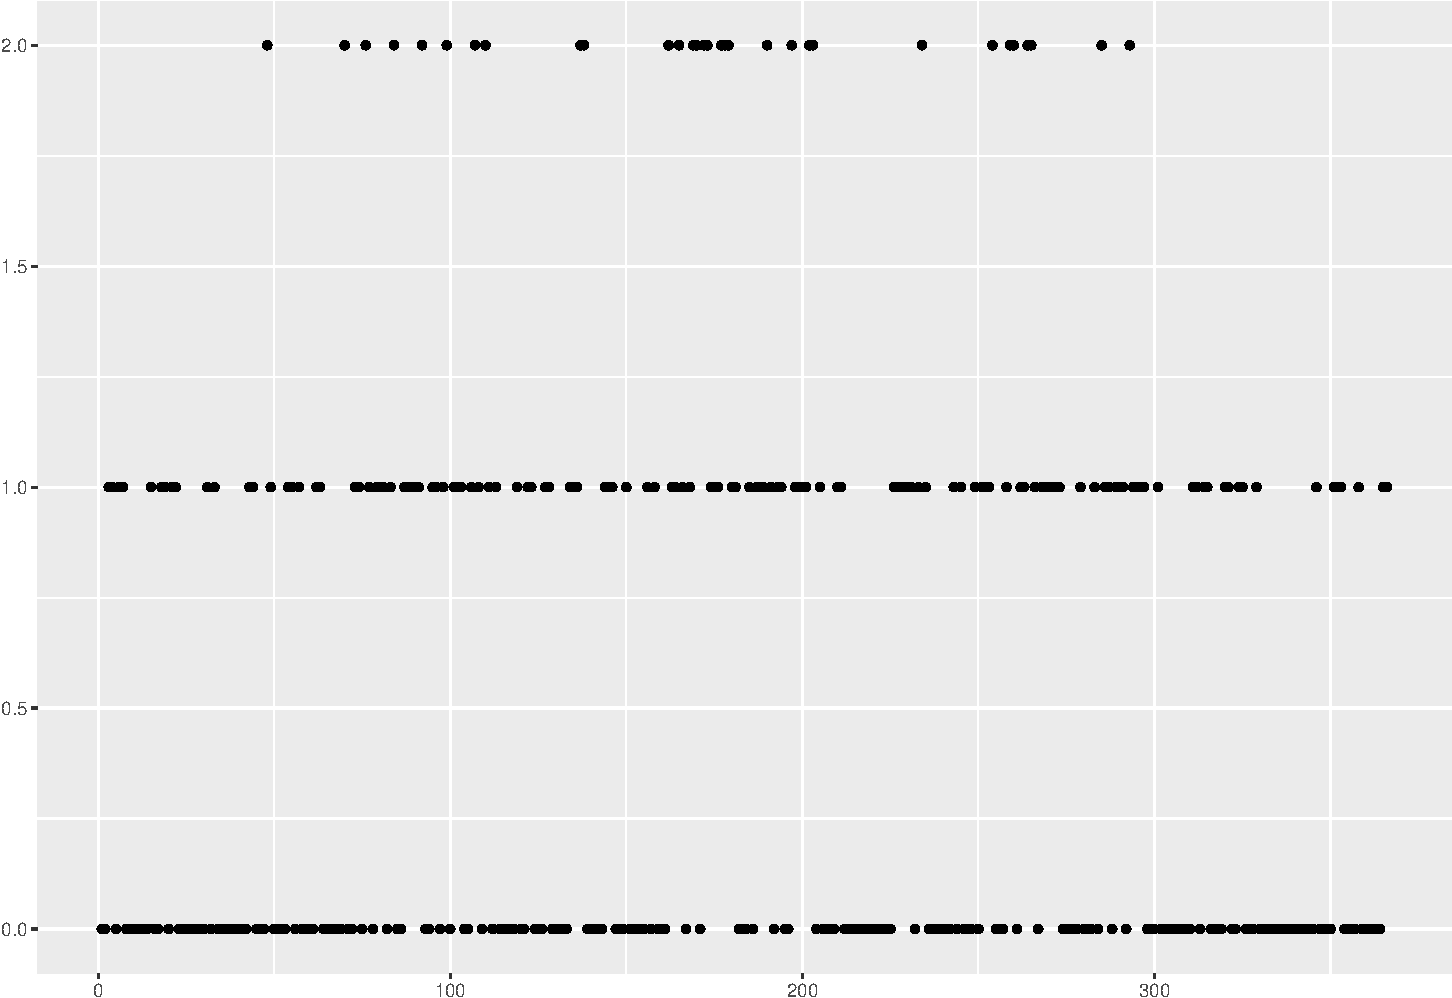
\includegraphics[width=0.6\linewidth]{Part4_Advanced_files/figure-beamer/unnamed-chunk-8-1} \end{center}
\normalsize
\end{frame}

\begin{frame}[fragile]{Example: fit the model}
\protect\hypertarget{example-fit-the-model}{}
\begin{Shaded}
\begin{Highlighting}[]
\NormalTok{cmp }\OtherTok{\textless{}{-}}\NormalTok{ y }\SpecialCharTok{\textasciitilde{}}  \SpecialCharTok{{-}}\DecValTok{1} \SpecialCharTok{+} \FunctionTok{int}\NormalTok{(int,  }\AttributeTok{model =} \StringTok{"factor\_full"}\NormalTok{) }\SpecialCharTok{+}
  \FunctionTok{myar1}\NormalTok{(t, }\AttributeTok{model =} \StringTok{"ar1"}\NormalTok{, }\AttributeTok{replicate =}\NormalTok{ repl)}
\NormalTok{fit }\OtherTok{\textless{}{-}} \FunctionTok{bru}\NormalTok{(cmp, }\AttributeTok{family =} \StringTok{"poisson"}\NormalTok{, }\AttributeTok{data =}\NormalTok{ df\_groups)}
\end{Highlighting}
\end{Shaded}
\end{frame}

\begin{frame}{Example: Results - Latent field}
\protect\hypertarget{example-results---latent-field}{}
\begin{center}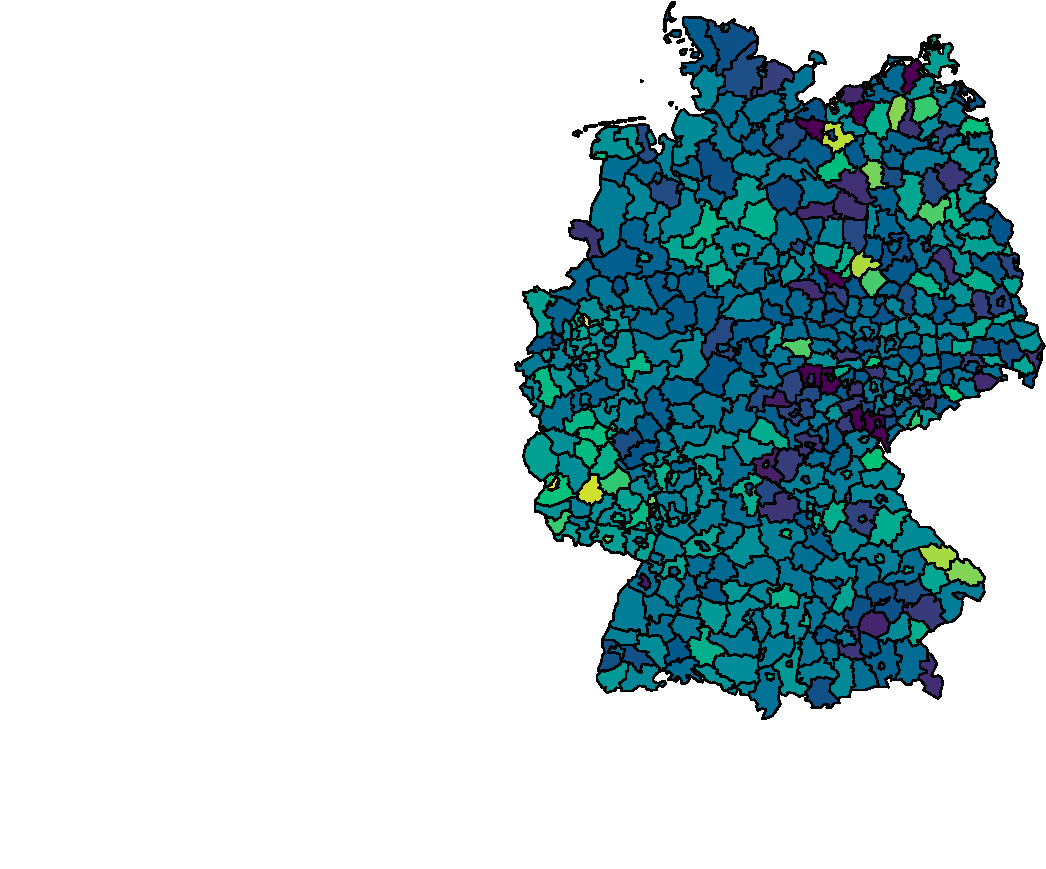
\includegraphics[width=0.8\linewidth]{Part4_Advanced_files/figure-beamer/unnamed-chunk-10-1} \end{center}
\end{frame}

\begin{frame}{Example: Results - Hyperparameters}
\protect\hypertarget{example-results---hyperparameters}{}
\begin{center}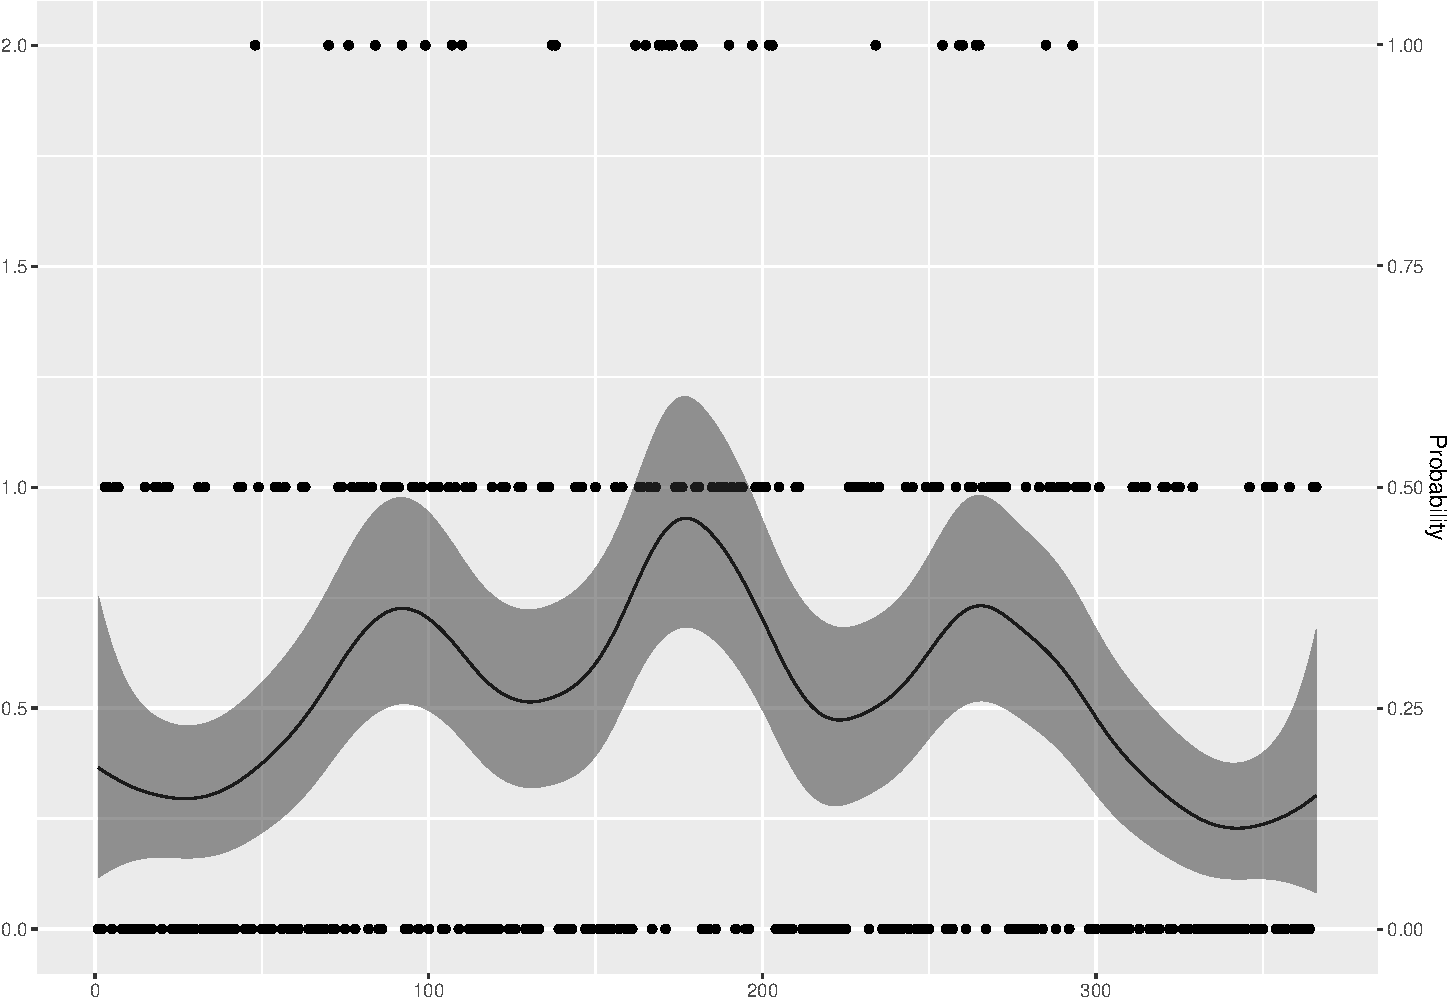
\includegraphics[width=0.6\linewidth]{Part4_Advanced_files/figure-beamer/unnamed-chunk-11-1} \end{center}
\end{frame}

\hypertarget{featuregroup}{%
\section{Feature:Group}\label{featuregroup}}

\begin{frame}[fragile]{Feature: \texttt{group}}
\protect\hypertarget{feature-group}{}
\begin{itemize}
\item
  Similar concept as replicate, but with a dependence structure on the
  replicates. E.g.\textasciitilde rw1, rw2, ar1, exchangeable
\item
  Implemented as a Kronecker product (often space and time)
\item
  It's possible to use both replicate and group! This will be
  replications of the grouped model
\item
  Usage
\end{itemize}

\begin{Shaded}
\begin{Highlighting}[]
    \FunctionTok{f}\NormalTok{(..., }\AttributeTok{group =}\NormalTok{ g [, }\AttributeTok{ngroup =}\NormalTok{ ng])}
\end{Highlighting}
\end{Shaded}

where replicate are integers \(1, 2, \ldots,\) etc
\end{frame}

\hypertarget{featuremultiple-likelihoods}{%
\section{Feature:Multiple
likelihoods}\label{featuremultiple-likelihoods}}

\begin{frame}{Feature:Multiple likelihood}
\protect\hypertarget{featuremultiple-likelihood}{}
There is no constraint in INLA that the type of likelihood must be the
same for all observations. In fact, every observation could have its own
likelihood.

\begin{itemize}
\item
  Coregionalization model
\item
  Marked point process
\item
  Joint models of various kinds
\end{itemize}
\end{frame}

\begin{frame}{Example: Simulate data}
\protect\hypertarget{example-simulate-data-2}{}
We fit a simple model where we imagine that some data come from a
Gaussian and some from a Poisson likelihood: \tiny

\normalsize
\end{frame}

\begin{frame}[fragile]{Example: Fit the model}
\protect\hypertarget{example-fit-the-model-1}{}
\begin{Shaded}
\begin{Highlighting}[]
\NormalTok{cmp }\OtherTok{=} \ErrorTok{\textasciitilde{}} \FunctionTok{Intercept\_1}\NormalTok{(}\DecValTok{1}\NormalTok{) }\SpecialCharTok{+} \FunctionTok{Intercept\_2}\NormalTok{(}\DecValTok{1}\NormalTok{) }\SpecialCharTok{+}
  \FunctionTok{x1}\NormalTok{(x1, }\AttributeTok{model =} \StringTok{"linear"}\NormalTok{) }\SpecialCharTok{+} \FunctionTok{x2}\NormalTok{(x2, }\AttributeTok{model =} \StringTok{"linear"}\NormalTok{)}

\NormalTok{lik1 }\OtherTok{=} \FunctionTok{like}\NormalTok{(}\AttributeTok{formula =}\NormalTok{ y1}\SpecialCharTok{\textasciitilde{}}\NormalTok{Intercept\_1 }\SpecialCharTok{+}\NormalTok{ x1,}
            \AttributeTok{family =} \StringTok{"gaussian"}\NormalTok{,}
            \AttributeTok{exclude =} \FunctionTok{c}\NormalTok{(}\StringTok{"Intercept\_2"}\NormalTok{,}\StringTok{"x2"}\NormalTok{),}
            \AttributeTok{data =}\NormalTok{ d1)}

\NormalTok{lik2 }\OtherTok{=} \FunctionTok{like}\NormalTok{(}\AttributeTok{formula =}\NormalTok{ y2}\SpecialCharTok{\textasciitilde{}}\NormalTok{Intercept\_2 }\SpecialCharTok{+}\NormalTok{ x2,}
            \AttributeTok{family =} \StringTok{"poisson"}\NormalTok{,}
            \AttributeTok{exclude =} \FunctionTok{c}\NormalTok{(}\StringTok{"Intercept\_1"}\NormalTok{,}\StringTok{"x1"}\NormalTok{),}
            \AttributeTok{data =}\NormalTok{ d2)}

\NormalTok{fit }\OtherTok{=} \FunctionTok{bru}\NormalTok{(cmp, lik1,lik2)}
\end{Highlighting}
\end{Shaded}
\end{frame}

\hypertarget{feature-copy}{%
\section{\texorpdfstring{Feature:
\texttt{copy}}{Feature: copy}}\label{feature-copy}}

\begin{frame}[fragile]{Feature: \texttt{copy}}
\protect\hypertarget{feature-copy-1}{}
\begin{verbatim}
Allows different elements of the same `f(...)` to be
in the the same linear predictor.
\end{verbatim}

\hfill\break

\begin{verbatim}
Without copy we can not (directly) specify the model
\end{verbatim}

\[
        \eta_i = u_i + u_{i+1} + \dots
\]

\hfill\break
Sometimes this is necessary
\end{frame}

\begin{frame}[fragile]{Feature: \texttt{copy}}
\protect\hypertarget{feature-copy-2}{}
\begin{verbatim}
The linear predictor
\end{verbatim}

\[
\eta_i = u_i + u_{i+1} + \ldots
\] can be coded as

\begin{Shaded}
\begin{Highlighting}[]
\NormalTok{   formula }\OtherTok{=}\NormalTok{ y }\SpecialCharTok{\textasciitilde{}} \FunctionTok{f}\NormalTok{(i, }\AttributeTok{model =} \StringTok{"iid"}\NormalTok{)}
                 \SpecialCharTok{+} \FunctionTok{f}\NormalTok{(i.plus, }\AttributeTok{copy=}\StringTok{"i"}\NormalTok{) }\SpecialCharTok{+}\NormalTok{ ...}
\end{Highlighting}
\end{Shaded}

\begin{itemize}
\item
  The copy-feature, creates internally an additional sub-model which is
  \(\epsilon\)-close to the target
\item
  Many copies allowed, and copies of copies
\end{itemize}
\end{frame}

\begin{frame}[fragile]{Feature: \texttt{copy}}
\protect\hypertarget{feature-copy-3}{}
\begin{verbatim}
It is also possible to include scaled copies
\end{verbatim}

\[
        \eta_i = u_i + \beta u_{i+1} + \ldots
\]

\hfill\break

\begin{Shaded}
\begin{Highlighting}[]
\NormalTok{   formula }\OtherTok{=}\NormalTok{ y }\SpecialCharTok{\textasciitilde{}} \FunctionTok{f}\NormalTok{(i, }\AttributeTok{model=}\StringTok{"iid"}\NormalTok{) }\SpecialCharTok{+}
                 \FunctionTok{f}\NormalTok{(i.plus, }\AttributeTok{copy=}\StringTok{"i"}\NormalTok{,}
                   \AttributeTok{hyper =} \FunctionTok{list}\NormalTok{(}\AttributeTok{beta=}\FunctionTok{list}\NormalTok{(}\AttributeTok{fixed=}\ConstantTok{FALSE}\NormalTok{)))}
                 \SpecialCharTok{+}\NormalTok{ ...}
\end{Highlighting}
\end{Shaded}

This introduces another hyperparameter in the model ( which is fixed to
1 by default).
\end{frame}

\begin{frame}{Feature: \texttt{copy}}
\protect\hypertarget{feature-copy-4}{}
\[
\begin{aligned}
y^1_i & \sim \mathcal{N}(\mu_i,\tau)\\
\mu_i &= f(i)\\
\\
y^2_j & \sim \text{Poisson}(\lambda_j),& j = 1,\dots,50\\
\log(\lambda_j) &= f(i)\\
\end{aligned}
\]
\end{frame}

\begin{frame}[fragile]{Example : simulate data}
\protect\hypertarget{example-simulate-data-3}{}
\footnotesize

\begin{Shaded}
\begin{Highlighting}[]
\NormalTok{n }\OtherTok{=} \DecValTok{50}
\NormalTok{idx }\OtherTok{=} \DecValTok{1}\SpecialCharTok{:}\NormalTok{n}
\NormalTok{x }\OtherTok{=}\NormalTok{ idx}
\NormalTok{func }\OtherTok{=} \DecValTok{10} \SpecialCharTok{*}\NormalTok{ ((idx}\SpecialCharTok{{-}}\NormalTok{n}\SpecialCharTok{/}\DecValTok{2}\NormalTok{)}\SpecialCharTok{/}\NormalTok{n)}\SpecialCharTok{\^{}}\DecValTok{3}

\NormalTok{y1 }\OtherTok{=} \FunctionTok{rnorm}\NormalTok{(}\DecValTok{50}\NormalTok{, }\AttributeTok{mean =}\NormalTok{ func, }\AttributeTok{sd =} \FloatTok{0.2}\NormalTok{)}
\NormalTok{y2 }\OtherTok{=} \FunctionTok{rpois}\NormalTok{(}\DecValTok{50}\NormalTok{, }\AttributeTok{lambda  =} \FunctionTok{exp}\NormalTok{(func))}
\end{Highlighting}
\end{Shaded}

\begin{center}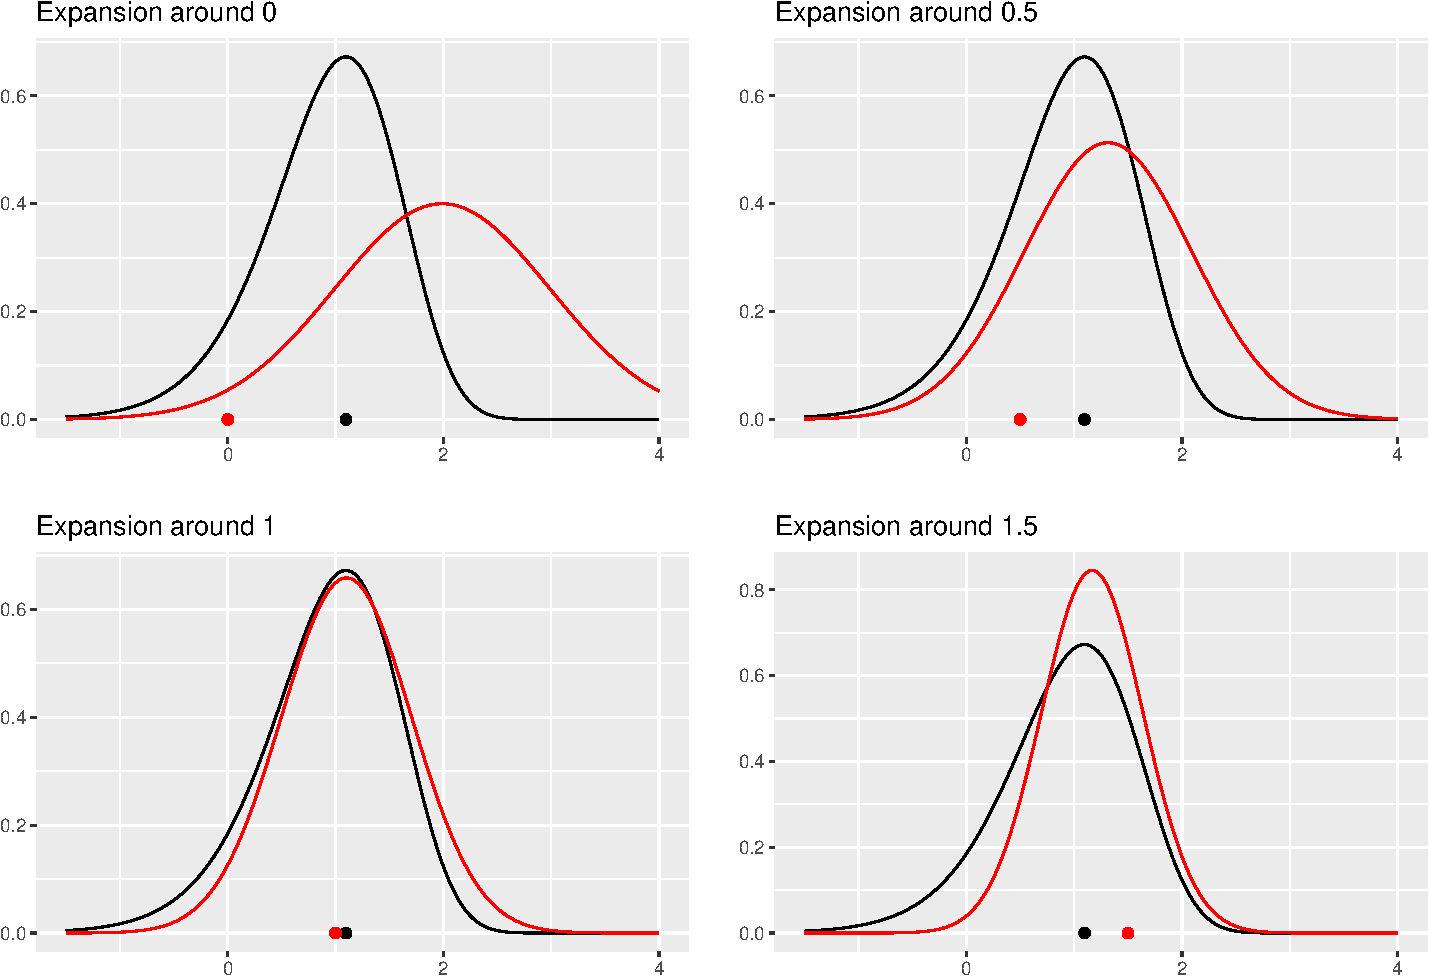
\includegraphics[width=0.6\linewidth]{Part4_Advanced_files/figure-beamer/unnamed-chunk-18-1} \end{center}
\normalsize
\end{frame}

\begin{frame}[fragile]{Example : fit the model}
\protect\hypertarget{example-fit-the-model-2}{}
\footnotesize

\begin{Shaded}
\begin{Highlighting}[]
\NormalTok{df1 }\OtherTok{=} \FunctionTok{data.frame}\NormalTok{(}\AttributeTok{y1 =}\NormalTok{ y1, }\AttributeTok{idx1 =}  \DecValTok{1}\SpecialCharTok{:}\NormalTok{n)}
\NormalTok{df2 }\OtherTok{=} \FunctionTok{data.frame}\NormalTok{(}\AttributeTok{y2 =}\NormalTok{ y2, }\AttributeTok{idx2 =}  \DecValTok{1}\SpecialCharTok{:}\NormalTok{n)}

\NormalTok{cmp }\OtherTok{=} \ErrorTok{\textasciitilde{}} \SpecialCharTok{{-}}\DecValTok{1} \SpecialCharTok{+} 
  \FunctionTok{field}\NormalTok{(idx1, }\AttributeTok{model =} \StringTok{"rw1"}\NormalTok{) }\SpecialCharTok{+} 
  \FunctionTok{field\_copy}\NormalTok{(idx2, }\AttributeTok{copy =} \StringTok{"field"}\NormalTok{)}

\NormalTok{lik1 }\OtherTok{=} \FunctionTok{like}\NormalTok{(}\AttributeTok{formula  =}\NormalTok{ y1}\SpecialCharTok{\textasciitilde{}}\NormalTok{ field,}
            \AttributeTok{family =} \StringTok{"gaussian"}\NormalTok{,}
            \AttributeTok{exclude =} \FunctionTok{c}\NormalTok{(}\StringTok{"field\_copy"}\NormalTok{),}
            \AttributeTok{data =}\NormalTok{ df1)}

\NormalTok{lik2 }\OtherTok{=} \FunctionTok{like}\NormalTok{(}\AttributeTok{formula  =}\NormalTok{ y2}\SpecialCharTok{\textasciitilde{}}\NormalTok{ field\_copy,}
            \AttributeTok{family =} \StringTok{"poisson"}\NormalTok{,}
            \AttributeTok{exclude =} \FunctionTok{c}\NormalTok{(}\StringTok{"field"}\NormalTok{),}
            \AttributeTok{data =}\NormalTok{ df2)}

\NormalTok{fit }\OtherTok{=} \FunctionTok{bru}\NormalTok{(cmp, }
\NormalTok{          lik1,}
\NormalTok{          lik2)}
\end{Highlighting}
\end{Shaded}

\normalsize
\end{frame}

\begin{frame}{Example: Results}
\protect\hypertarget{example-results}{}
\begin{center}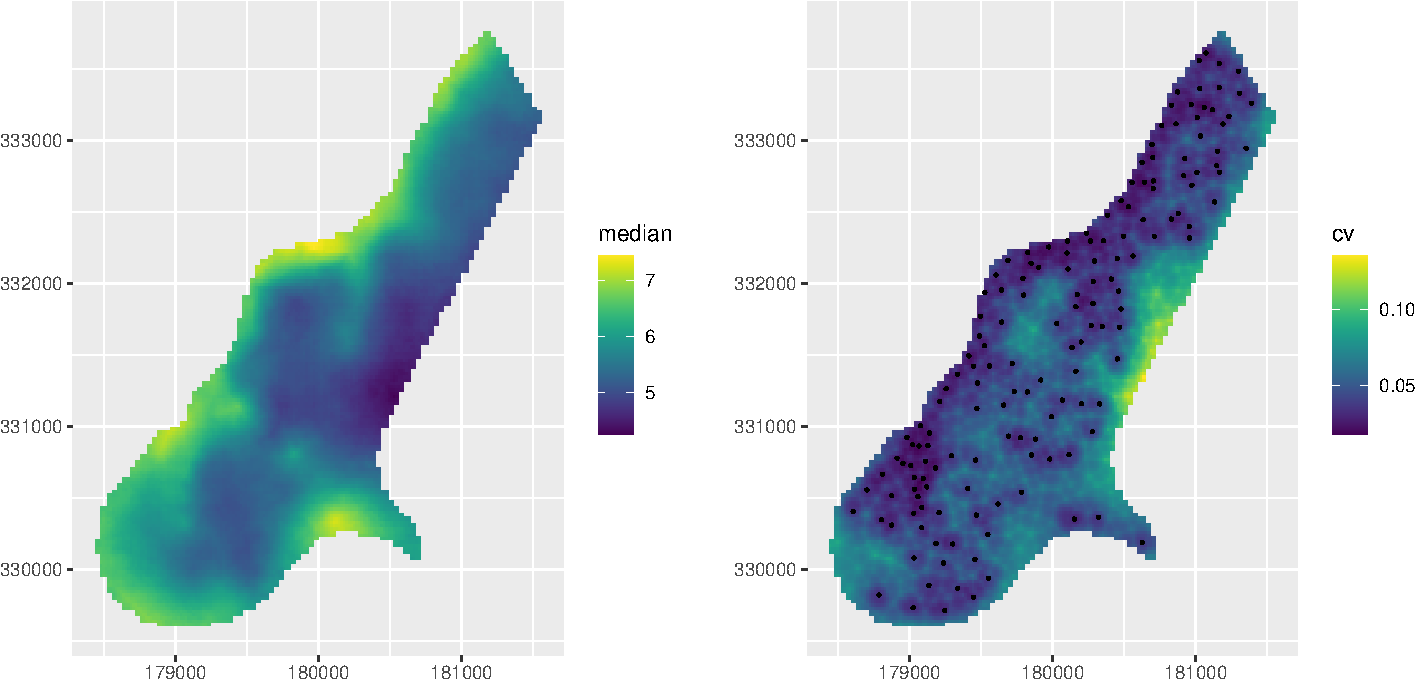
\includegraphics[width=0.6\linewidth]{Part4_Advanced_files/figure-beamer/unnamed-chunk-20-1} \end{center}
\end{frame}

\end{document}
